\documentclass{beamer}
\usetheme{default}
\usepackage{amsmath}
\usepackage{tabularx}
\usepackage{booktabs}
\usepackage{colortbl}
\usepackage{tikz}
\usetikzlibrary{calc}
\pgfdeclarelayer{background}
\pgfdeclarelayer{foreground}
\pgfsetlayers{background,main,foreground}
\setbeamertemplate{background canvas}[vertical shading]%
  [top=blue!1,bottom=blue!30]
\setbeamertemplate{navigation symbols}{}
\newcommand*\up{\textcolor{green}{%
  \ensuremath{\blacktriangle}}}
\newcommand*\down{\textcolor{red}{%
  \ensuremath{\blacktriangledown}}}
\newcommand*\const{\textcolor{darkgray}{\textbf{--}}}

\begin{document}
\begin{frame}[bg=lightgray]
\textbf{\Large Linux distribution ranking, 26th August 2009}
\begin{center}
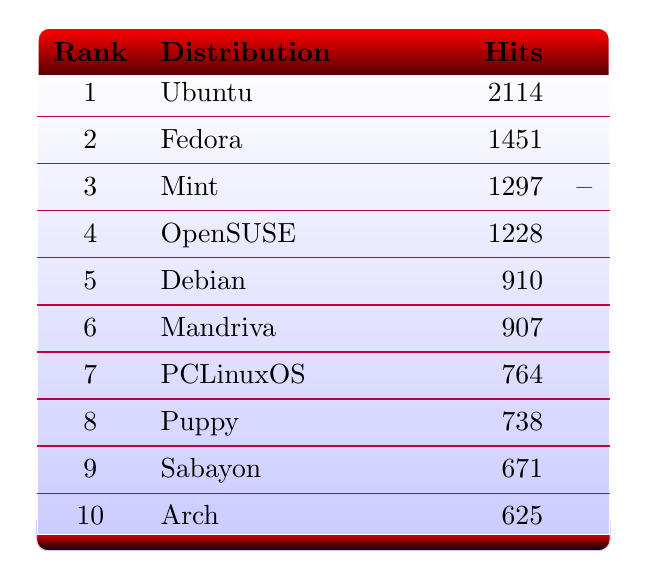
\begin{tikzpicture}
\node (tbl) {
\begin{tabularx}{.6\textwidth}{cXrcc}
\arrayrulecolor{purple}
\textbf{Rank} & \textbf{Distribution} & \textbf{Hits} & \\
1 & Ubuntu\rule{0pt}{2.5ex}  &  2114 & \down \\
\midrule
2 & Fedora & 1451 & \up \\
\midrule
3 & Mint & 1297 & \const \\
\midrule
4 & OpenSUSE & 1228 & \up \\
\midrule
5 & Debian & 910 & \down \\
\midrule
6 & Mandriva & 907 & \up \\
\midrule
7 & PCLinuxOS & 764 & \up \\
\midrule
8 & Puppy & 738 & \up \\
\midrule
9 & Sabayon & 671 & \up \\
\midrule
10 & Arch & 625 & \down \\[0.5ex]
\end{tabularx}};
\begin{pgfonlayer}{background}
\draw[rounded corners,top color=red,bottom color=black,
    draw=white] ($(tbl.north west)+(0.14,0)$)
    rectangle ($(tbl.north east)-(0.13,0.9)$);
\draw[rounded corners,top color=white,bottom color=black,
    middle color=red,draw=blue!20] ($(tbl.south west)
    +(0.12,0.5)$) rectangle ($(tbl.south east)-(0.12,0)$);
\draw[top color=blue!1,bottom color=blue!20,draw=white]
    ($(tbl.north east)-(0.13,0.6)$)
    rectangle ($(tbl.south west)+(0.13,0.2)$);
\end{pgfonlayer}
\end{tikzpicture}
\end{center}
\small
Data by DistroWatch.com, spanning over the last 6 months,
hits per day.
\end{frame}
\end{document}
